\chapter{Estado de la Cuestión}
\label{cap:estadoDeLaCuestion}
Antes de empezar a diseñar la herramienta es necesario conocer lo que usan o lo que hacen normalmente las empresas actuales con la adaptación del videojuego a otros países o regiones. En este capitulo contaré que es la internacionalización, localización, LQA y errores lingüísticos comunes. Además necesitaremos una herramienta que nos permita obtener la información necesaria desde una imagen, para ello esta el OCR (\textit{Optical Character Recognition}), elegiremos y evaluaremos unas de ellas.

\section{Internacionalización}
\label{sec:Internacionalización}
La internacionalización es el proceso de preparar un producto para que pueda admitir diferentes idiomas y convenciones culturales sin necesidad de volver a rediseñarse.

Según \cite{LQAPSM2017}, la internacionalización de un videojuego implica una serie de decisiones técnicas y de diseño que permiten su adaptación posterior a múltiples idiomas y culturas sin necesidad de modificar su estructura principal. Esto implica separar la lógica de la aplicación de los elementos dependientes del idioma y de la cultura, como los textos, las fechas, las divisas, y otros formatos específicos. A continuación, se detallan algunos de los aspectos más relevantes según  \cite{LQAPSM2017}:
\begin{itemize}
	\item Separación del texto traducible de código fuente. Esto ayuda a que el traductor se centre únicamente en el trabajo de traducción y no tenga que acceder al código fuente.
	\item Uso de fuentes adecuadas para distintos idiomas. Las fuentes deben mostrar todos los posibles caracteres del idioma seleccionado, el fallo de esto puede conllevar a que en el videojuego no se vea el texto completo.
	\item Uso de la codificación adecuada para distintos idiomas.Según \cite{Codificacion} la codificación es la forma en que se traduce la información para que pueda ser interpretada y utilizada por una máquina.La mala elección o uso de la codificación puede provocar que se genere caracteres no legibles como se muestra en la figura \ref{fig:EFontC}, al igual que el uso incorrecto de la fuente donde la fuente no incluye algún carácter que se esta utilizando ,por tanto es necesario que la codificación pueda interpretar un carácter o símbolo introducido por teclado. Se usa el estándar de Unicode.
	\item Diseño de interfaces adaptables al texto que se debe mostrar. La misma cadena de texto en distintos idiomas traducidos pueden necesitar distintos espacios para mostrarlo en pantalla, esto puede conllevar a un problema a la hora de diseñar la interfaz y el espacio que tiene en el videojuego para mostrar una cadena.
	\cite{LQAPSM2017} plantea las siguientes posibilidades de solucionar el problema:
	
	\begin{itemize}
		\item Uso de fuente de ancho variable siempre que sea posible. La fuente elegida afecta mucho a la hora de mostrar más o menos caracteres. Existen las fuentes de ancho fija (todos los caracteres ocupan exactamente el mismo número de píxeles), fuentes de ancho variable (cada carácter ocupa un determinado número de píxeles). Poner ejemplos.
		\item Uso de bocadillos, cajas o ventanas de texto adaptables al contenido. El tamaño de las ventanas se adaptará al tamaño de texto que hay dentro.
		\item Uso de menús y botones con gran espacio o adaptables al contenido. En muchas ocasiones surge el problema de que el texto traducido no quepa en el espacio del botón o del menú, para ello se recomienda que se hagan con espacio suficiente para abordar cualquier posible tamaño de la traducción o que sean adaptables al contenido.
	\end{itemize}
	\item Uso de etiquetas especiales para marcar género, sexo o número. Un problema a la hora de traducir reside en la concordancia de género, sexo y número en distintos idiomas, un ejemplo es \textit{``You are so nice''} se puede traducir como ``Eres muy simpático'' o ``Eres muy simpática''. Por lo tanto es necesario la existencia de un sistema que cambie la palabra según si se trata de un personaje masculino o femenino.
	
	\item Facilitación de un mínimo de información contextual. En distintos idiomas puede resultar que la traducción sea diferente dependiendo del contexto, esto el traductor no lo sabe, por lo tanto es necesario un mínimo de información contextual para agilizar el proceso de traducción.
	
	\item Comprobación cultural de imágenes e iconos. Algunos gestos, imágenes o iconos pueden resultar inapropiados para algunas culturas o religiones hay que tener especial cuidado con la zona de localización.
\end{itemize}
	\begin{figure}[H]
	\centering
	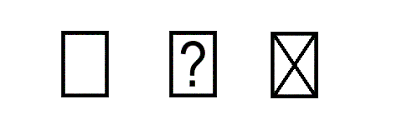
\includegraphics[width = 0.5\textwidth]{Imagenes/Errores_Localizacion/E_Font_C.png}
	\caption{Glifos con lo que se representa comúnmente cuando hay error de fuente.}
	\label{fig:EFontC}
\end{figure}

\section{Localización}
\label{sec:Localization}

Según el articulo de \cite{Localization}, la \textbf{Localización} (o L10N), es el proceso por el cuál un producto se adapta a un idioma y/o cultura diferente del idioma o cultura en el que el producto fue creado satisfaciendo las necesidades. Esto incluye, pero no se limita, a la traducción de los textos y audios. 

En el contexto de los videojuegos, la localización es esencial para proporcionar una experiencia inmersiva y auténtica a los jugadores de diferentes regiones. Esto incluye la adaptación de referencias culturales, chistes, juegos de palabras y otros elementos lingüísticos que podrían no tener un significado directo en el idioma de destino. Por ejemplo, si un videojuego contiene juegos de palabras complejos, el localizador debe encontrar equivalentes adecuados en el nuevo idioma que transmitan el mismo efecto o emoción, en lugar de realizar una traducción literal.

Además, la localización puede abarcar aspectos como la adaptación de símbolos, iconos, colores y otros elementos visuales que puedan tener connotaciones diferentes en diversas culturas. También es importante considerar las diferencias en formatos de fecha, hora, monedas y unidades de medida para garantizar que el producto sea completamente funcional y comprensible para el usuario final. 

\section{Localization Quality Assurance}
\label{sec:LQA}

Según \cite{QA}, QA (\textit{Quality Assurance}) es un proceso sistemático para garantizar que un producto o servicio cumpla con los requisitos de calidad establecidos.
No se trata de probar un producto, sino de prevenir errores y defectos a lo largo del proceso de desarrollo.
Esto ayuda al aumento de la confianza de los usuarios, a la vez ayuda al proceso y la eficiencia del desarrollo.

En cuanto LQA (\textit{Localization Quality Assurance}) según \cite{LQA} es un proceso esencial en la localización de contenido que garantiza que el producto adaptado sea preciso, funcional y culturalmente apropiado para su mercado objetivo. A diferencia de la simple corrección de textos, LQA evalúa el contenido en su contexto real, considerando aspectos lingüísticos, visuales, funcionales y culturales.

\begin{itemize}
\item Lingüístico: Verifica la precisión de la traducción, la gramática, la ortografía y la coherencia terminológica.
\item Visual: Asegura que el texto traducido se visualice correctamente en la interfaz, sin desbordamientos ni problemas de formato.
\item Funcional: Comprueba que todas las funciones del producto operen según lo esperado en el idioma de destino.
\item Cultural y legal: Evalúa que el contenido sea apropiado culturalmente y cumpla con las normativas legales del mercado objetivo.

\end{itemize}

Integrar LQA en el flujo de trabajo de localización desde las etapas iniciales permite identificar y corregir problemas oportunamente, mejorando la eficiencia y reduciendo costos. Herramientas como Gridly facilitan este proceso al centralizar la gestión de contenido y permitir colaboraciones en tiempo real entre desarrolladores, traductores y testers. Además proporciona control de versiones, revisión contextual donde puede comprobar como se vería por ejemplo un botón con el texto si encaja o no, validación automática de reglas donde puedes definir validaciones como longitud máximo del texto, uso consistente de mayúsculas, prohibición de ciertos términos.



\section{Errores de localización comunes}
\label{sec:Errores de localizacion}
Según \cite{LQAPSM2017} existe numerosos errores de localización en los videojuegos a continuación se describirá cada uno de ellos.

\subsection{Problema de fuente} \label{ErrorFuente}
Este error se da comúnmente cuando la fuente utilizada en el videojuego no incluye algunos caracteres especiales de un idioma, como puede ser la ñ en español o caracteres del chino, normalmente se presentan como se muestra en la figura \ref{fig:EFontC}
Un ejemplo podría ser como se muestra en la figura \ref{fig:EFont} donde algunos caracteres chinos no se muestran correctamente. 

\begin{figure}[H]
	\centering
	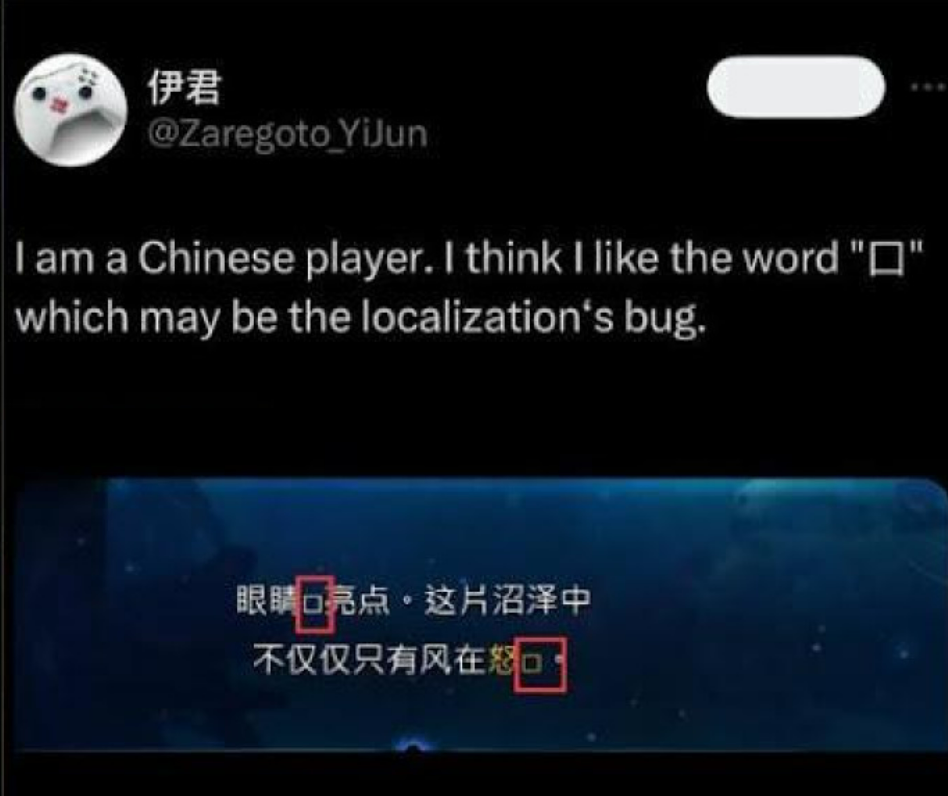
\includegraphics[width = 0.5\textwidth]{Imagenes/Errores_Localizacion/E_Font.png}
	\caption{Twitter de un jugador chino que reporta un error en la fuente del juego.}
	\label{fig:EFont}
\end{figure}

\subsection{Implementación de texto incorrecta}\label{ErrorImpIncorrecta}
Este error se ilustra cuando el texto que debería aparecer en un idioma, aparece en otro diferente o aparece en forma de ``placeholder''(Figura \ref{fig:E_Implementacion}). Este error se produce debido a que hay un error en el documento de localización o porque el programa en sí tiene algún error. Debido a esto, el \textit{tester} tiene que verificar que la celda del documento tiene el
texto adecuado.
\begin{figure}[H]
	\centering
	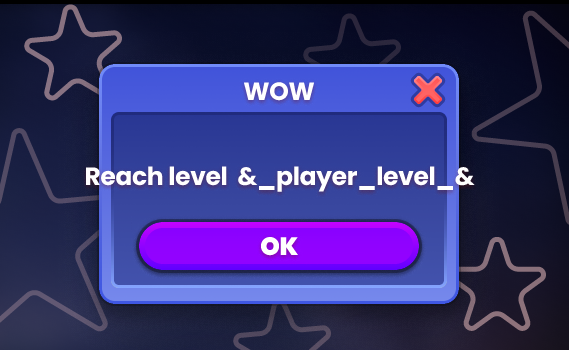
\includegraphics[width = 0.5\textwidth]{Imagenes/Errores_Localizacion/E_Implementacion.png}
	\caption{Aparece un placeholder en vez del nivel alcanzado}
	\label{fig:E_Implementacion}
\end{figure}
\subsection{Cadena no localizada}\label{ErrorNoLocalizada}
Este error se produce cuando un texto no está traducido como se muestra en la figura \ref{fig:EImplementacion_Incorrecta}. Esto puede ocurrir cuando el traductor no haya traducido el texto o que el desarrollador no haya proporcionado el texto. 
\begin{figure}[H]
	\centering
	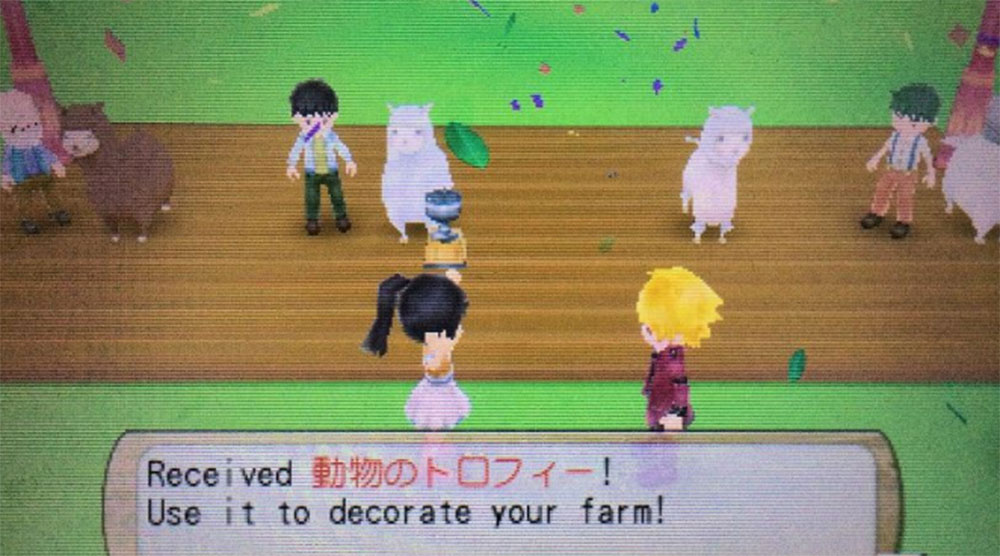
\includegraphics[width = 0.5\textwidth]{Imagenes/Errores_Localizacion/E_Implementacion_Incorrecta.png}
	\caption{Parte del texto se queda sin ser traducido.}
	\label{fig:EImplementacion_Incorrecta}
\end{figure}

\subsection{Error tipográfico o de ortografía}\label{ErrorTypo}
Surge cuando existe alguna falta de ortografía en el texto traducido. Por ejemplo en el juego de GhostBusters, los jugadores se encuentran con ``Conglatulation'' donde lo correcto sería ``Congratulations'' como se muestra en la figura \ref{fig:E_Tipo}
\begin{figure}[H]
	\centering
	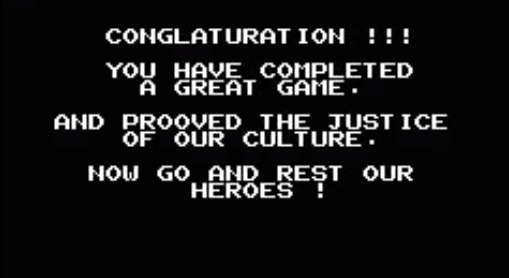
\includegraphics[width = 0.5\textwidth]{Imagenes/Errores_Localizacion/E_Tipo.png}
	\caption{Error tipográfico en el juego de GhostBusters.}
	\label{fig:E_Tipo}
\end{figure}
\subsection{Error gramatical}\label{ErrorGramatical}
Surge cuando existe un fallo gramatical en el texto traducido. Es necesario tener un conocimiento perfecto del idioma al que se traduce.Un ejemplo sería como se muestra en la figura \ref{fig:EGrammar} donde el personaje dice ``Did something happened?'', en lugar de ``Did something happen?'' que sería lo correcto.
\begin{figure}[H]
	\centering
	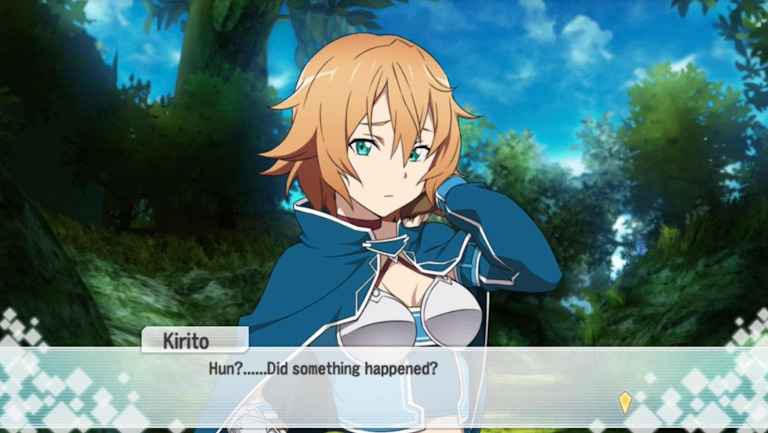
\includegraphics[width = 0.5\textwidth]{Imagenes/Errores_Localizacion/E_Grammar.png}
	\caption{Error gramatical en ingles del juego.}
	\label{fig:EGrammar}
\end{figure}

\subsection{Error de traducción}\label{ErrorTraducción}
Este error se da cuando el texto traducido es errónea(p.ej ``Dinero'' traducido a ``monkey'' en lugar de ``money''). Este error es uno de los errores más importantes ya que dar información incorrecta al jugador implica dar una experiencia desastrosa al jugador.
Suele ocurrir cuando es mal traducido, por falta de información u omisión de palabras o que no tenga sentido en el contexto. Un ejemplo es como se muestra en la figura \ref{fig:ETraduccion} donde \textit chest puede ser traducido como ``cofre'' o ``pecho'' dependiendo del contexto, en este caso la traducción al chino ha sido pecho en vez de cofre.
\begin{figure}[H]
	\centering
	
\includegraphics[width = 0.5\textwidth]{Imagenes/Errores_Localizacion/E_Traduccion.png}
	\caption{Mal traducción de cofre (\textit{chest}) al chino.}
	\label{fig:ETraduccion}
\end{figure}

\subsection{Solapamiento de texto}\label{ErrorSolapamiento}
Este error sucede cuando el texto se sale de los limites fijados para él, puede ser un botón o un cuadro de texto. Puede deberse por una mala implementación por parte del desarrollador o que el traductor no haya respetado los límites de espacios proporcionado.(Figura \ref{fig:E_Solapa})
\begin{figure}[H]
	\centering
	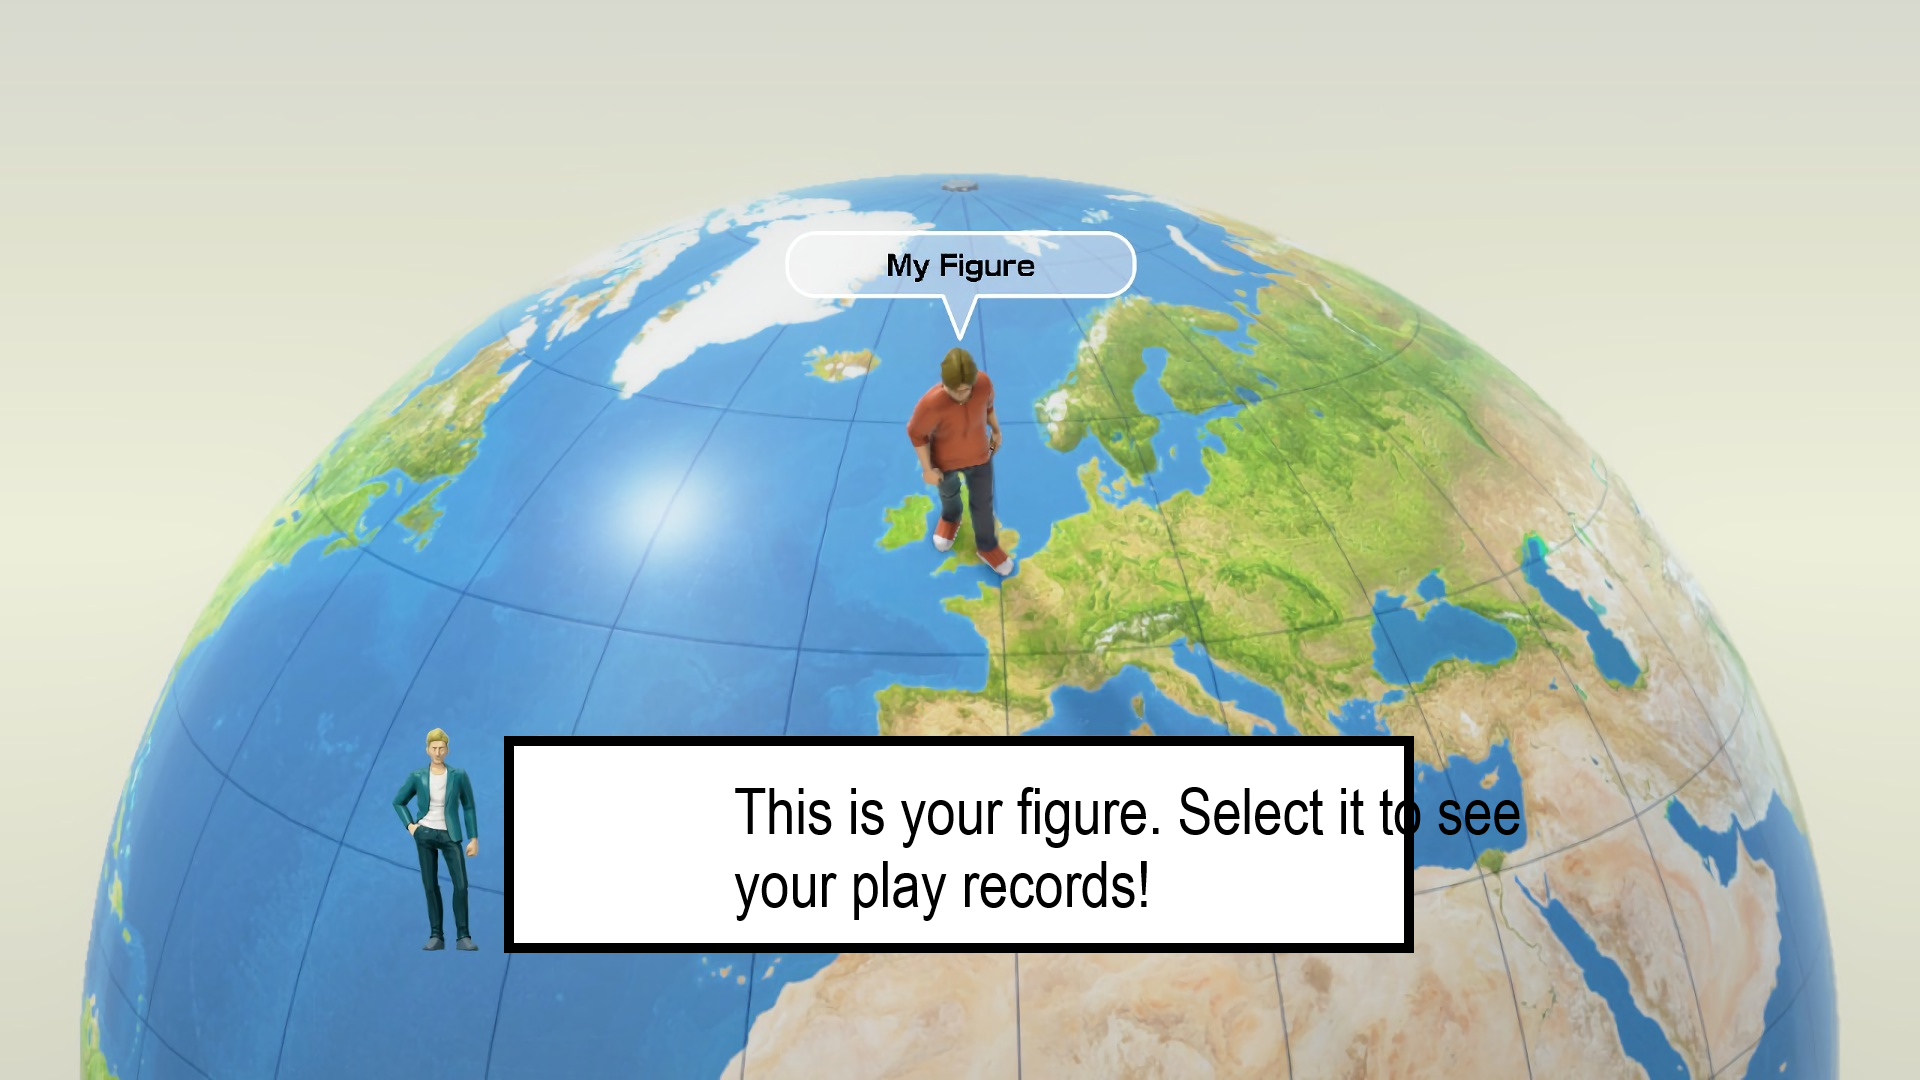
\includegraphics[width = 0.5\textwidth]{Imagenes/Errores_Localizacion/E_Solapamiento.png}
	\caption{El texto sobresale de la caja delimitadora.}
	\label{fig:E_Solapa}
\end{figure}

\subsection{Truncamiento de texto}\label{ErrorTruncamiento}
Este error se produce cuando un texto aparece cortado y no se muestra por completo. Puede deberse a que no haya suficiente espacio dentro de los limites fijados.
(Figura \ref{fig:E_Trunc})
\begin{figure}[H]
	\centering
	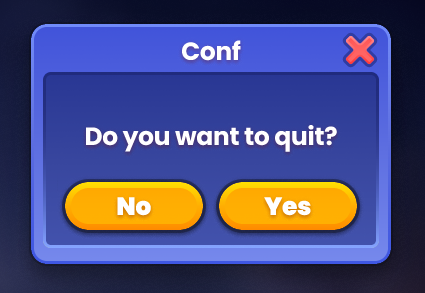
\includegraphics[width = 0.5\textwidth]{Imagenes/Errores_Localizacion/E_Trunca.png}
	\caption{El texto confirm no aparece completo.}
	\label{fig:E_Trunc}
\end{figure}

\subsection{Error terminológico o incoherencia}\label{ErrorTermino}
Este error se produce cuando se usa una palabra incorrecta para referirse a una
terminología clave (p. ej. utilizar el término ``grabar'' en lugar de ``guardar''). También
puede darse cuando el mismo término no está escrito de la misma manera en dos
lugares distintos (p. ej. Escribir un término importante en minúsculas en un lugar
y en mayúsculas en otro.).
Un ejemplo podría ser que en la descripción se describa como un tipo de daño, sin embargo, en el efecto aparezca otro como se muestra en la figura \ref{fig:EIncoherencia}.
\begin{figure}[H]
	\centering
	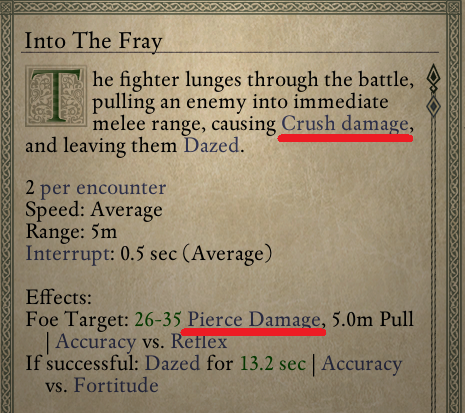
\includegraphics[width = 0.5\textwidth]{Imagenes/Errores_Localizacion/E_Incoherencia.png}
	\caption{Incoherencia entre la descripción y el efecto.}
	\label{fig:EIncoherencia}
\end{figure}

\subsection{Incumplimiento de directrices}\label{ErrorDirectrices}
Este error se da cuando una traducción no se cumplen las reglas de estilo que
impone un distribuidor o plataforma para los videojuegos que se publiquen en ella.
Por ejemplo, los mensajes del sistema en videojuegos en consolas deben de escribirse
exactamente como aparecen en las TRC (\textit{Technical Requirements Checklist}) de la compañía.

\subsection{Error de subtítulos}\label{ErrorSubtitulos}
Los subtitulos pueden tener diferentes error, los más comunes son los siguientes:
\begin{itemize}
	\item Los subtitulos no aparecen.
	\item Los subtitulos aparecen desincronizados
	\item Subtitulos muy largos por lo que no da tiempo leer.
	\item No estar bien segmentados como se muestra en la figura \ref{fig:ESubtitulo}
	\item No coinciden con el audio doblado.
\end{itemize}
\begin{figure}[H]
	\centering
	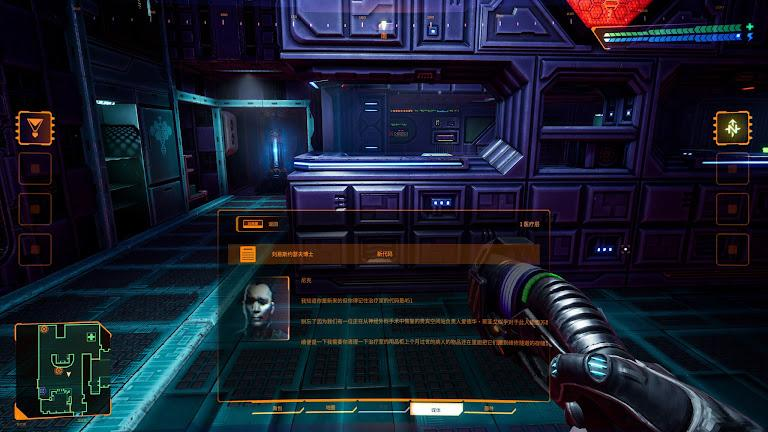
\includegraphics[width = 0.5\textwidth]{Imagenes/Errores_Localizacion/E_Subtitulo.png}
	\caption{Falta de segmentación por lo que dificulta la lectura.}
	\label{fig:ESubtitulo}
\end{figure}
\subsection{Error de audio}\label{ErrorAudio}

Al igual que los subtitulos, los errores de audio puede ser de varios tipos:
\begin{itemize}
	\item El dialogo no esta doblado o no se escucha
	\item El audio esta desincronizado
	\item El audio no coincide con el contexto.
\end{itemize}

\subsection{Problemas culturales}\label{ErrorCultura}
Este error se suele dar cuando en un videojuego se utiliza alguna simbología
o gesto que tiene un significado ofensivo en otra cultura. Un ejemplo puede ser la
utilización del símbolo manji en un juego japonés, que es muy parecido a la esvástica
de la Alemania nazi como aparece en la figura \ref{fig:ManjiEsvastica}.
\begin{figure}[H]
	\centering
	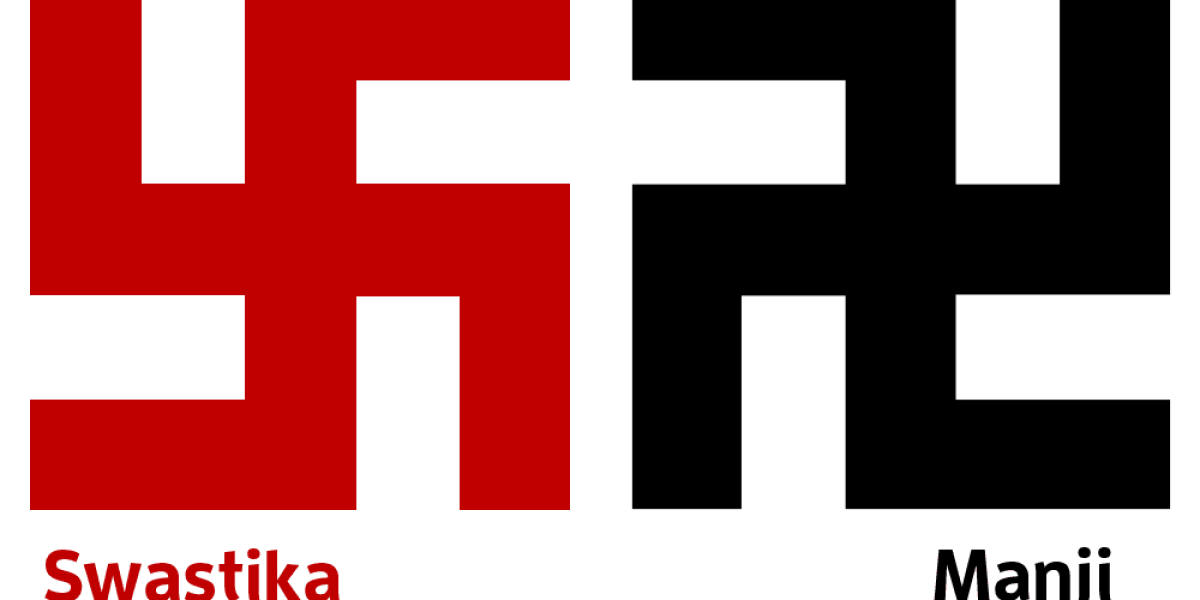
\includegraphics[width = 0.5\textwidth]{Imagenes/Errores_Localizacion/manji-swastika.png}
	\caption{Diferencia entre manji y esvástica.}
	\label{fig:ManjiEsvastica}
\end{figure}


\section{Reconocimiento Óptico de Caracteres (OCR)}
El OCR (Reconocimiento Óptico de Caracteres, por sus siglas en inglés \textit{Optical Character Recognition}) es una tecnología que convierte imágenes de texto manuscrito, impreso o mecanografiado en datos de texto que las computadoras pueden interpretar y manipular según \cite{WhatIsOCR}. En otras palabras, puede extraer el texto contenida en una imagen. Según \cite{WhatIsOCR} el OCR se usa en varios sectores:
\begin{itemize}
	\item El sector bancario utiliza el OCR para procesar y verificar el papeleo de documentos de préstamo, cheques de depósito y otras transacciones financieras.
	\item El sector de la salud utiliza el OCR para procesar registros de pacientes, incluidos tratamientos, pruebas, registros hospitalarios y pagos de seguros.
	\item Las empresas de logística utilizan el OCR para rastrear etiquetas de paquetes, facturas, recibos y otros documentos de manera más eficiente. 
\end{itemize}


Según \cite{TesseractOCR} y \cite{OcropusOCR} para llegar al objetivo de reconocer el texto y extraerlo de la imagen el OCR da una serie de pasos:
\begin{enumerate}
	\item \textbf{Preprocesamiento de la imagen:}
	
	El propósito de este paso es procesar la imagen para que sea más legible para la computadora y reconocer así de forma mas eficiente los textos.
	\begin{itemize}
		\item Conversión a escala de grises: La mayoría de los OCR primero convierten la imagen en blanco y negro o escala de grises para simplificar el procesamiento.
		\item Reducción de ruido: Se aplican filtros para eliminar manchas, borrones o marcas en la imagen que puedan afectar la precisión del reconocimiento.
		\item Binarización: La imagen se convierte a una representación en blanco y negro, donde los píxeles se clasifican como parte del fondo (blanco) o del texto (negro). Este proceso ayuda a aislar los caracteres.
	\end{itemize}
	
	\item \textbf{Segmentación:}
	
	El OCR divide la imagen en secciones manejables. Primero separa líneas de texto.  Luego separa las palabras y finalmente descompone las palabras en caracteres individuales. Este paso es crucial, ya que el OCR necesita reconocer los caracteres de manera individual, pero considerando también su contexto dentro de una palabra o frase.
	
	\item \textbf{Detección de características:}
	
	Extracción de características de los caracteres: El OCR analiza los caracteres y sus formas, midiendo varios atributos como las líneas, contornos, cruces de líneas, y la disposición de los píxeles. Estos datos son usados para diferenciar letras, números y símbolos similares (como ``O'' y ``0'' o ``l'' y ``1'').
	Se aplican técnicas basadas en modelos geométricos, estructuras de redes neuronales o de aprendizaje automático para identificar patrones comunes en los caracteres.
	
	\item \textbf{Reconocimiento del carácter:}
	
	Una vez identificadas las características, el OCR las compara con una base de datos o ``alfabeto'' interno de posibles caracteres. Esto puede hacerse de varias maneras según \cite{WhatIsOCR}, dependiendo del tipo de OCR:
	\begin{itemize}
		\item Métodos basados en plantillas: Se compara cada carácter con un conjunto de plantillas predefinidas. Si la forma del carácter coincide con una plantilla, se clasifica como ese carácter.
		\item Métodos basados en aprendizaje automático o redes neuronales: Las técnicas modernas de OCR suelen usar redes neuronales entrenadas con miles de ejemplos de texto. El sistema ``aprende'' a identificar caracteres y a hacer distinciones más sutiles en base a sus experiencias pasadas.
	\end{itemize}
\end{enumerate}
\subsection{Librerías de OCR}
\label{subsec:Seleccion de libreria de OCR}
Durante el desarrollo de este trabajo, se evaluarán varias herramientas de OCR para seleccionar la más adecuada para nuestras necesidades. Las herramientas que probaremos serán OCRopus\footnote{Repositorio github de OCRopus:  \url{https://github.com/ocropus-archive/DUP-ocropy} }, EasyOCR\footnote{Repositorio github de EasyOCR:  \url{https://github.com/JaidedAI/EasyOCR} } y Tesseract\footnote{Repositorio github de Tesseract:  \url{https://github.com/tesseract-ocr/tesseract} }. A continuación, se describe brevemente cada una de ellas.
\begin{enumerate}
	\item \textbf{OCRopus}
	Es un sistema de OCR basado en redes neuronales con un enfoque modular.
	Principalmente esta disponible para Linux. Proporciona diferentes módulos para la binarización, segmentación, generación del ground-truth y el entreno del modelo.
	La última actualización de esta librería fue en 16 de Diciembre de 2017
	
	\item \textbf{EasyOCR}
	EasyOCR es una biblioteca de reconocimiento óptico de caracteres (OCR) desarrollada en Python que facilita la extracción de texto de imágenes y documentos. Diseñada con el objetivo de ser fácil de usar y accesible, una de las características de EasyOCR es que es capaz de reconocer texto en más de 80 idiomas y soporta múltiples scripts, lo que la convierte en una herramienta versátil para diversas aplicaciones.
	Proporciona gran variedad de modelos entrenados y también ofrece la opción de entrenar tu propio modelo.
	
	La herramienta en resumen se adapta muy bien a nuestras necesidades.
	
	\item \textbf{Tesseract}
	
	Tesseract es una biblioteca de (OCR) de código abierto que se utiliza para convertir imágenes de texto en texto editable. Originalmente desarrollado por Hewlett-Packard en la década de 1980, Tesseract fue liberado como software de código abierto en 2005 y ha sido mantenido y mejorado por la comunidad, particularmente por Google, que ha contribuido significativamente a su desarrollo.
	
	Al igual que EasyOCR una de las características más destacadas de Tesseract es su capacidad para reconocer texto en múltiples idiomas y alfabetos, soportando más de 100 idiomas de forma nativa. Esto lo convierte en una herramienta versátil para aplicaciones globales que requieren la extracción de texto de documentos escritos en diferentes lenguas.
	
	Tesseract utiliza técnicas avanzadas de aprendizaje profundo y redes neuronales, lo que le permite alcanzar altos niveles de precisión en el reconocimiento de texto. Su arquitectura se basa en el uso de modelos de aprendizaje profundo entrenados con grandes conjuntos de datos, lo que mejora continuamente su rendimiento en diversas condiciones.
	
	El motor puede integrarse fácilmente en aplicaciones de procesamiento de imágenes y visión por computadora. Tesseract se utiliza comúnmente en combinación con bibliotecas como OpenCV para preprocesar imágenes antes de la etapa de reconocimiento, lo que mejora la precisión de los resultados.
	
	Además, Tesseract ofrece una API en varios lenguajes de programación, lo que facilita su integración en diferentes entornos de desarrollo.
\end{enumerate}
\section{Conclusión}
En conclusión, la internacionalización trata de preparar el producto para que sea fácilmente admitir diferentes idiomas y para ello es necesario seguir algunas pautas como la separación del texto traducible de código fuente. La localización es el proceso por la cual un producto se adapta a un cierto idioma o cultura, esto es esencial en videojuegos para que los jugadores de otras regiones tengan una experiencia inmersiva y auténtica. QA(\textit{Quality Assurance}) se trata de un proceso sistemático para garantizar que un producto cumpla los requisitos y LQA(\textit{Localization Quality Assurance}) es el mismo proceso centrándose en aspectos de la localización como los aspectos lingüísticos, visuales, funcionales y culturares. El OCR es una tecnología que consigue convertir imágenes con texto en datos de texto que la computadora pueda entender.

Esta sección contribuye a comprender el funcionamiento de un sistema OCR, así como la existencia de errores de localización que deben ser resueltos. Además, se analiza cómo se representan visualmente estos errores en pantalla, lo que resulta fundamental para el diseño de las distintas partes de la herramienta tanto los tests como el propio OCR que se detallan en el siguiente capítulo.
